\documentclass[12pt]{article}

% ---------- Packages ----------
\usepackage[margin=1in]{geometry}
\usepackage{graphicx}
\usepackage{tikz}
\usetikzlibrary{arrows.meta,positioning}

\usepackage{listings}
\usepackage{xcolor}
\usepackage{amsmath}
\usepackage{booktabs}
\usepackage[english]{babel}
\usepackage{csquotes}
\usepackage[backend=biber,style=apa]{biblatex}
\addbibresource{reference.bib}
\usepackage[hidelinks]{hyperref}
\usepackage{xurl}
%\usepackage{cleveref}
\usepackage{caption}
\usepackage{titlesec}
\usepackage{fontspec}
\setmainfont{Times New Roman}
\usepackage{setspace}
\onehalfspacing
\usepackage{tocloft}
\usepackage{float}   % for [H] figure placement
\usepackage{tabularx}
\usepackage{array}

\graphicspath{{../outputs/figures/}}

%% ---------- Custom Email ----------

\makeatletter
\newcommand{\email}[1]{%
    \begingroup
    \def\UrlBreaks{\do\@\do\.}% Only allow breaks at @ and .
    \def\UrlBigBreaks{}%
    \def\UrlNoBreaks{}%
    \def\UrlOrds{}% Clear xurl's default breaks after letters/numbers
    \href{mailto:#1}{\nolinkurl{#1}}%
    \endgroup
}
\makeatother

% ---------- Code listing style (for Python code blocks) ----------
\lstdefinestyle{python}{
    language=Python,
    basicstyle=\ttfamily\small,
    keywordstyle=\color{blue},
    commentstyle=\color{gray},
    stringstyle=\color{teal},
    numbers=left,
    numberstyle=\tiny\color{gray},
    frame=single,
    breaklines=true,
    showstringspaces=false,
    tabsize=4
}
\lstset{style=python}

\lstdefinestyle{compact}{
    language=Python,
    basicstyle=\ttfamily\scriptsize,   % smaller than \small
    keywordstyle=\color{blue},
    commentstyle=\color{gray},
    stringstyle=\color{teal},
    numbers=left,
    numberstyle=\tiny\color{gray},
    frame=single,
    breaklines=true,
    showstringspaces=false,
    tabsize=2,
    columns=fullflexible,
    xleftmargin=1em
}

% ---------- Cover page color (adjust RGB to match your exact previous shade if needed) ----------
\definecolor{blue-x}{HTML}{4472C4}

% Optional: nicer listing names
\renewcommand{\lstlistlistingname}{List of Listings}
\renewcommand{\lstlistingname}{Listing}

% Skip indentation for paragraphs but keep in between spacing
\setlength{\parindent}{0pt}
\setlength{\parskip}{0.5\baselineskip}

% Control section heading and spacing
\titleformat{\section}
{\normalfont\Large\bfseries}
{\thesection}
{1em}
{}

\titlespacing*{\section}
{0pt}{2.0ex}{0.8ex}

\titleformat{\subsection}
{\normalfont\large\bfseries}
{\thesubsection}
{1em}
{}

\titlespacing*{\subsection}
{0pt}{1.5ex}{0.6ex}

\titleformat{\subsubsection}
{\normalfont\normalsize\bfseries}
{\thesubsubsection}
{1em}
{}

\titlespacing*{\subsubsection}
{0pt}{1.2ex}{0.4ex}

% Shell/PowerShell listing style (no Python keywords, no line numbers)
\lstdefinestyle{shell}{
    style=python,
    language={},
    numbers=none,
    keywordstyle={},
    commentstyle={},
    stringstyle={},
    postbreak=\mbox{\textcolor{gray}{$\hookrightarrow$}\space}
}

% \shot{path}{caption}{label}
\newcommand{\shot}[3]{%
    \begin{figure}[htbp]
        \centering
        \includegraphics[width=\linewidth,height=0.38\textheight,keepaspectratio]{#1}
        \caption{#2}\label{#3}
\end{figure}}

% \shotpair{path1}{path2}{caption}{label}  (two stacked images, one caption)
\newcommand{\shotpair}[4]{%
    \begin{figure}[H]
        \centering
        \includegraphics[width=\linewidth,height=0.30\textheight,keepaspectratio]{#1}\\[6pt]
        \includegraphics[width=\linewidth,height=0.30\textheight,keepaspectratio]{#2}
        \caption{#3}\label{#4}
\end{figure}}

\begin{document}

%%%%%%%%%%%%%%%%%%%%%%%%%%%%%%%%%%%%%%
% COVER PAGE
%%%%%%%%%%%%%%%%%%%%%%%%%%%%%%%%%%%%%%

\begin{titlepage}
    \centering
    {\singlespacing\fontsize{20pt}{22pt}\selectfont\textbf{\textcolor{blue-x}{Large-Scale Analysis and Prediction of Building Electricity Consumption Using Weather and Building Characteristics}}\par}

    \vfill

    {\large\textbf{\underline{WM\_ASDS19: Big Data (Section: A)}}}\\[8pt]
    {\large\textbf{Spring 2026}}\\[8pt]
    {\large\textbf{Submission Date: 27 November 2026}}

    \vfill

    
\includegraphics{ju_logo.jpg}

    \vfill

    {\fontsize{18pt}{20pt}\selectfont\textbf{\textcolor{blue-x}{Submitted by}}}
    \vspace{8pt}

    {\fontsize{14pt}{16pt}\selectfont Group Name: \textbf{Data Explorers}}\\[8pt]
    {\fontsize{14pt}{16pt}\selectfont Group Members ID: 20251702, 20251703, 20251717, 20251739}

    \vfill

    {\fontsize{18pt}{20pt}\selectfont\textbf{\textcolor{blue-x}{Submitted to}}}

    \vspace{8pt}

    {\fontsize{14pt}{16pt}\selectfont Farhana Akter Bina}\\[8pt]
    {\fontsize{14pt}{16pt}\selectfont Associate Professor}

    \vfill

    {\fontsize{18pt}{20pt}\selectfont\textbf{\textcolor{blue-x}{Department of Statistics \& Data Science}}}\\[8pt]

    {\fontsize{18pt}{20pt}\selectfont\textbf{\textcolor{blue-x}{Jahangirnagar University}}}
\end{titlepage}

\clearpage

\begingroup

% Suppress page numbers throughout the front matter
\pagestyle{empty}

% Also suppress page numbers on pages that force the 'plain' style
\makeatletter
\let\ps@plain\ps@empty
\makeatother

% Table of Contents
%\begingroup
%\setlength{\cftbeforesecskip}{8pt}
\tableofcontents
%\endgroup
\clearpage

% List of Figures
\listoffigures
% \clearpage

% List of Tables
\listoftables

% List of Listings
%\lstlistoflistings
\clearpage

\endgroup

% Restore page numbering for the main report
\pagestyle{plain}

% =========================================================
\section{Introduction}
% =========================================================

\subsection{Background and Motivation}

Buildings consume substantial amounts of electricity for lighting, heating, ventilation, air conditioning, and the operation of electrical equipment. Understanding and predicting electricity consumption is important for efficient energy management, demand planning, and reducing operational costs.

The increasing adoption of smart meters and automated building monitoring systems has enabled the collection of large volumes of energy consumption data. When combined with building characteristics and meteorological observations, these data provide opportunities to investigate consumption patterns and develop data-driven predictive models~\parencite{miller2020building}.

However, processing millions of observations presents computational challenges, particularly when working with limited memory and computing resources. Big Data processing technologies and computationally efficient machine learning algorithms can help address these challenges.

\subsection{Problem Statement}

Building electricity consumption varies across buildings, time periods, and weather conditions. These variations may result from differences in building size, functionality, operating schedules, and environmental conditions. The relationships among these factors and electricity consumption may be nonlinear and involve complex interactions.

This study uses the ASHRAE Great Energy Predictor III dataset to develop a large-scale electricity consumption prediction framework. Particular emphasis is placed on investigating whether weather variables provide additional predictive information beyond building characteristics and temporal factors.

The study also examines the relative importance of individual predictors and demonstrates the reproducibility of the data-processing and modeling workflows using alternative data-processing approaches.

\subsection{Objectives}

The main objectives of this study are:

\begin{itemize}
    \item To develop an efficient data-processing workflow for large-scale building electricity consumption data.

    \item To investigate temporal, building-specific, and weather-related electricity consumption patterns.

    \item To develop and evaluate a LightGBM-based model for predicting hourly electricity consumption.

    \item To assess the additional predictive value of weather variables.

    \item To evaluate the relative importance of individual predictors and feature groups using gain-based feature importance.

    \item To independently verify the data-processing and model-fitting workflows using PySpark-generated data.
\end{itemize}

% =========================================================
\section{Dataset Description}
% =========================================================

\subsection{Data Source}

The dataset was obtained from the ASHRAE Great Energy Predictor III competition on Kaggle~\parencite{ashrae}. The complete competition package contains six uncompressed CSV files totaling 2.61~GB (2.43~GiB). The competition used part of the Building Data Genome Project 2, a broader collection of hourly energy measurements from non-residential buildings across 19 sites in North America and Europe~\parencite{miller2020building}.

The three raw files processed in this study totaled 686.11~MB (654.33~MiB). They contain labeled meter readings (\nolinkurl{train.csv}), building metadata (\nolinkurl{building_metadata.csv}), and training weather (\nolinkurl{weather_train.csv}). The December holdout comes from the labeled meter readings.

\subsection{Dataset Characteristics}

The original training dataset contains 20,216,100 hourly meter observations across four meter categories: electricity, chilled water, steam, and hot water.

This study focuses on electricity consumption (meter = 0), which initially contains 12,060,910 observations.

The building metadata provides information such as building type, site identification, and floor area. Weather data includes air temperature, dew-point temperature, and wind speed.

\subsection{Description of Variables}

The predictive model uses ten input variables representing building characteristics, temporal factors, and weather conditions, with hourly electricity consumption as the target variable.

The building-use classifications follow the ENERGY STAR property-type definitions~\parencite{miller2020building}. Temporal variables were derived from the original timestamp. \autoref{tab:variable_description} summarizes the variables used in the predictive model.

\begin{table}[htbp]
    \centering
    \caption{Description of Variables Used in Predictive Modeling}
    \label{tab:variable_description}

    \begingroup
    \small
    \renewcommand{\arraystretch}{1.4}
    \setlength{\tabcolsep}{5pt}

    \begin{tabularx}{\textwidth}{
            l
            l
            c
            >{\raggedright\arraybackslash}X
        }
        \toprule
        \textbf{Variable} &
        \textbf{Type} &
        \textbf{Unit} &
        \textbf{Description} \\
        \midrule

        \multicolumn{4}{l}{\textit{Building Characteristics}} \\

        \texttt{building\_id} & Categorical & -- &
        Unique building identifier. \\

        \texttt{site\_id} & Categorical & -- &
        Identifier of the building's site. \\

        \texttt{primary\_use} & Categorical & -- &
        Primary building-use category based on
        ENERGY STAR property-type definitions. \\

        \texttt{square\_feet} & Numerical & ft$^2$ &
        Gross floor area of the building. \\

        \midrule
        \multicolumn{4}{l}{\textit{Temporal Variables}} \\

        \texttt{hour} & Discrete & -- &
        Hour of the day (0--23). \\

        \texttt{day\_of\_week} & Discrete & -- &
        Day of the week (0 for Sunday through 6 for Saturday). \\

        \texttt{month} & Discrete & -- &
        Month of the year (1--12). \\

        \midrule
        \multicolumn{4}{l}{\textit{Weather Variables}} \\

        \texttt{air\_temperature} & Numerical & $^\circ$C &
        Outdoor air temperature. \\

        \texttt{dew\_temperature} & Numerical & $^\circ$C &
        Temperature at which air becomes saturated
        with water vapor. \\

        \texttt{wind\_speed} & Numerical & m/s &
        Outdoor wind speed. \\

        \midrule
        \multicolumn{4}{l}{\textit{Target Variable}} \\

        \texttt{meter\_reading} & Numerical & kWh &
        Recorded hourly electricity consumption, excluding Site 0. \\

        \bottomrule
    \end{tabularx}
    \endgroup
\end{table}

% =========================================================
\section{Methodology}
% =========================================================

\subsection{Big Data Processing Framework}

DuckDB was used for the primary data processing workflow, including data inspection, filtering, joining, aggregation, and preparation of model-ready data.

PySpark was independently used to reproduce the preprocessing workflow and verify the resulting dataset statistics. The processed data were stored in Apache Parquet format for efficient subsequent analysis.

\autoref{fig:project-workflow} summarizes the steps from raw data to holdout evaluation.

\begin{figure}[H]
    \centering
    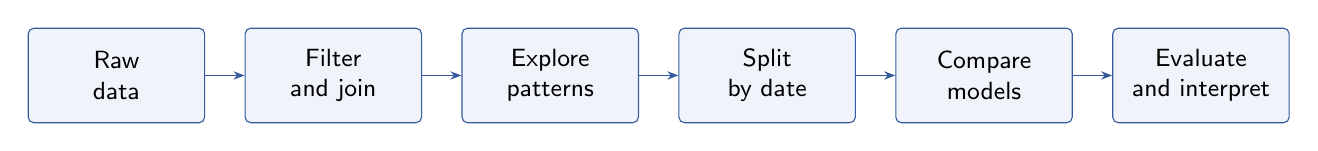
\begin{tikzpicture}[
        node distance=5mm,
        stage/.style={
            draw=blue-x!80!black,
            fill=blue-x!8,
            rounded corners=2pt,
            text width=21mm,
            minimum height=12mm,
            align=center,
            inner xsep=2pt,
            font=\small\sffamily
        },
        flow/.style={-{Stealth[length=4pt]}, semithick, draw=blue-x!80!black}
    ]
    \node[stage] (input) {Raw\\data};
    \node[stage, right=of input] (clean) {Filter\\and join};
    \node[stage, right=of clean] (explore) {Explore\\patterns};
    \node[stage, right=of explore] (split) {Split\\by date};
    \node[stage, right=of split] (models) {Compare\\models};
    \node[stage, right=of models] (test) {Evaluate\\and interpret};
    \draw[flow] (input) -- (clean);
    \draw[flow] (clean) -- (explore);
    \draw[flow] (explore) -- (split);
    \draw[flow] (split) -- (models);
    \draw[flow] (models) -- (test);
\end{tikzpicture}

    \caption{Main steps in the electricity prediction study,
    including model evaluation and feature importance analysis.}
    \label{fig:project-workflow}
\end{figure}

\subsection{Data Preprocessing}

Site 0 was excluded from the electricity analysis because of prolonged periods of anomalous zero readings and a documented difference in measurement units. The ASHRAE competition documentation identifies Site 0 electricity readings as being in kBTU~\parencite{ashrae}. After excluding Site 0, the analysis treated the remaining electricity readings as kWh throughout.

\autoref{fig:site-zero} shows how the share of zero electricity readings at Site 0 varied by month.

\shot{monthly_percentage_of_zero_electricity_readings_site0.png}
{Monthly share of zero electricity readings at Site 0 in 2016.}
{fig:site-zero}

After filtering and integrating the relevant datasets, 11,152,501 electricity observations were retained.

\subsection{Data Integration and Feature Engineering}

Electricity readings were joined with building metadata using building identifiers. Weather observations were subsequently joined using site identifiers and timestamps.

Temporal variables, including hour, day of week, and month, were extracted from timestamps.

The building and calendar predictors were building ID, site ID, primary use, floor area, hour, day of week, and month. The weather predictors were air temperature, dew-point temperature, and wind speed.

Air-temperature observations were available for 99.58\% of the processed records.

\subsection{Exploratory Data Analysis}

Exploratory data analysis was conducted to investigate electricity consumption patterns across different hours, building categories, and weather conditions.

A weekday-by-hour heatmap was also developed using PySpark to examine the combined effect of weekday and hour on electricity consumption.

\subsection{Predictive Modeling}

Light Gradient Boosting Machine (LightGBM) was employed to predict hourly electricity consumption.

The target variable was transformed using:

\begin{equation}
    z = \ln(1+y)
\end{equation}

where $y$ represents the observed electricity meter reading.

Three predictive approaches were evaluated:
\begin{itemize}
    \item Historical building-hour median baseline.
    \item LightGBM without weather variables.
    \item LightGBM with weather variables.
\end{itemize}

The historical baseline predicted the training median for each building and hour of day. It used the building median for unseen building-hour pairs and the overall training median for unseen buildings.

Both LightGBM regressors used 200 boosting rounds, a learning rate of 0.05, a maximum of 31 leaves per tree, and 127 histogram bins. Building ID, site ID, and primary use were encoded as categorical features using the training data. Predictions were returned to the original scale with $\exp(\hat z)-1$ and clipped at zero. Both runs used the full training partition. The second run added the three weather predictors to measure their contribution under the same model settings.

\subsection{Training, Validation, and Testing}

A chronological data partitioning strategy was adopted to preserve the temporal ordering of observations.

\begin{itemize}
    \item Training: January--September 2016 (8,321,304 observations).
    \item Validation: October--November 2016 (1,887,642 observations).
    \item Testing: December 2016 (943,555 observations).
\end{itemize}

The model configuration was selected using validation RMSLE. December observations from the labeled training file were reserved for the final holdout evaluation.

\subsection{Evaluation Metrics}

Model performance was evaluated using Mean Absolute Error (MAE) and Root Mean Squared Logarithmic Error (RMSLE).

MAE measures the average absolute prediction error, while RMSLE evaluates prediction errors on a logarithmic scale.

For $n$ observations with actual readings $y_i$ and predictions $\hat y_i$,
\begin{align}
    \mathrm{MAE} &= \frac{1}{n} \sum_{i=1}^{n} |y_i-\hat y_i|, \\
    \mathrm{RMSLE} &= \sqrt{\frac{1}{n}\sum_{i=1}^{n}
    \bigl[\ln(1+y_i)-\ln(1+\hat y_i)\bigr]^2}.
\end{align}
Lower values indicate better predictive performance.

\subsection{Feature Importance}

Gain-based feature importance was extracted from the final
fitted LightGBM model without retraining.

For predictor $j$, the normalized gain was calculated as

\begin{equation}
    I_j =
    \frac{G_j}{\sum_{k=1}^{p} G_k}\times 100,
\end{equation}

where $G_j$ is its accumulated split gain and $p=10$ is
the number of predictors.

Group-wise importance was calculated by summing the
normalized gains of building, temporal, and weather
predictors. These measures describe contributions to the
training objective rather than statistical significance
or explained variance.

% =========================================================
\section{Practical Application}
\label{sec:practical-application}

A facilities team could use predicted hourly electricity consumption as a reference when reviewing meter data. For a given building and hour, the team could compare the measured reading with the model estimate and investigate persistent differences alongside operating schedules and weather conditions.

To demonstrate this workflow, the model application notebook loaded the saved LightGBM model with weather features and sampled five building-hour observations from the December 2016 holdout using a fixed random seed. It supplied the model with building, calendar, and weather features and kept the observed meter readings for comparison in \autoref{tab:application-predictions}.

\begin{table}[htbp]
    \centering
    \caption{Observed and predicted electricity readings for five December 2016 observations.}
    \label{tab:application-predictions}
    \begin{tabular}{llrr}
        \toprule
        Building ID & Date and hour & Observed (kWh) & Predicted (kWh) \\
        \midrule
        975 & 26 Dec., 13:00 & 257.00 & 456.67 \\
        965 & 26 Dec., 17:00 &  20.00 &  28.88 \\
        431 &  5 Dec., 14:00 &  12.95 &  17.27 \\
        510 & 22 Dec., 23:00 &   4.28 &   8.44 \\
        1324 &  7 Dec., 13:00 &  13.00 &  35.94 \\
        \bottomrule
    \end{tabular}
\end{table}

The model overpredicted all five readings in this sample. The largest difference occurred for building 975, where the prediction exceeded the observed reading by 199.67~kWh. An isolated difference can reflect model error or a change in building operations, so a facilities team would review several hours before drawing conclusions. The aggregate holdout metrics in \autoref{tab:test_results} summarize performance across the full December partition.

\section{Results and Analysis}
% =========================================================

\subsection{Hourly Electricity Consumption}

As shown in \autoref{fig:hourly}, the mean across buildings was lowest at 03:00 (139.42~kWh) and peaked at 14:00 (189.06~kWh). Each building contributes its mean reading for the given hour. The timing is consistent with higher electricity use during normal operating hours.

\shot{average_hourly_electricity_consumption.png}
{Mean electricity meter reading by hour of day.}
{fig:hourly}

\subsection{Electricity Consumption by Building Category}

To give each building equal weight within its category, we first calculated its mean hourly reading per 1,000 square feet, then averaged those values by primary use. \autoref{fig:building-use} shows categories with at least 20 buildings.

\shot{average_hourly_electricity_use_by_building_category.png}
{Mean hourly electricity reading per 1,000 square feet by primary use.}
{fig:building-use}

Healthcare buildings exhibited relatively high electricity consumption per 1,000 square feet, while residential buildings showed comparatively lower values.

These differences may reflect variations in building operations, occupancy, and energy requirements.

\subsection{Relationship Between Weather and Electricity Consumption}

\autoref{fig:temperature} shows mean electricity readings grouped into 2~$^\circ$C outdoor air temperature bins with at least 1,000 readings. The resulting pattern was nonlinear.

\shot{outdoor_temperature_and_electricity_consumption.png}
{Mean electricity meter reading by outdoor air temperature bin.}
{fig:temperature}

Higher average consumption was observed at very low temperatures, while consumption varied across warmer temperature ranges.

These descriptive relationships may also reflect differences in building characteristics and geographical locations.

\subsection{Weekday and Hourly Consumption Heatmap}

\autoref{fig:weekday-hour} shows mean electricity readings by day of week and hour of day. PySpark first calculated a mean for each building within each cell, then averaged across those buildings.

\shot{../validation/anik-pyspark/weekday_hour_heatmap.png}
{Mean electricity meter reading by day of week and hour of day.}
{fig:weekday-hour}

The highest mean reading occurred on Tuesday at 14:00, with approximately 204.85 kWh.

Daytime weekday consumption was generally higher than weekend consumption. Given the North American and European geographical coverage of the source data~\parencite{miller2020building}, this pattern is consistent with conventional Monday--Friday working schedules and potentially higher weekday occupancy and operational activity. Individual building schedules and public holidays were not explicitly accounted for.

\subsection{Validation Performance}

The validation results are summarized in \autoref{tab:validation_results}.

\begin{table}[htbp]
    \centering
    \caption{Validation performance of predictive models}
    \label{tab:validation_results}
    \begin{tabular}{lcc}
        \hline
        Model & MAE & RMSLE \\
        \hline
        Historical Baseline & 38.6666 & 0.8672 \\
        LightGBM without Weather & 41.0398 & 0.7225 \\
        LightGBM with Weather & 35.9330 & 0.6939 \\
        \hline
    \end{tabular}
\end{table}

LightGBM without weather lowered RMSLE relative to the historical baseline while increasing MAE. The model with weather achieved the lowest validation score on both metrics.

\subsection{Contribution of Weather Variables}

Including weather variables reduced validation RMSLE from 0.7225 to 0.6939, corresponding to an improvement of approximately 4.0\%.

Validation MAE also decreased from 41.0398 to 35.9330, representing an improvement of approximately 12.4\%.

These results suggest that weather observations provide useful additional information for predicting electricity consumption.

\subsection{Final Test Performance}

The selected LightGBM model was evaluated on 943,555 December observations. \autoref{tab:test_results} compares its performance with the historical baseline.

\begin{table}[htbp]
    \centering
    \caption{Final December test performance}
    \label{tab:test_results}
    \begin{tabular}{lcc}
        \hline
        Model & MAE & RMSLE \\
        \hline
        Historical Baseline & 44.9097 & 0.7756 \\
        LightGBM with Weather & 41.0866 & 0.6245 \\
        \hline
    \end{tabular}
\end{table}

The selected model reduced test RMSLE by approximately 19.5\% compared with the historical baseline, demonstrating improved predictive performance on the held-out month. \autoref{fig:actual-predicted} shows the agreement between actual and predicted readings, with the diagonal marking equal values.

\shot{actual_vs_predicted_electricity_prediction.png}
{Actual and predicted electricity readings for a sample of 10,000 December observations. The axes end at the pooled 99th percentile of actual and predicted readings.}
{fig:actual-predicted}

\subsection{Feature Importance Analysis}

\autoref{fig:feature-importance} presents the normalized
gain and split frequency of each predictor in the
selected LightGBM model.

\shot{lightgbm_feature_importance.png}
{Gain-based feature importance of the selected LightGBM
    model. The panels use different horizontal scales to
improve the visibility of lower-importance predictors.}
{fig:feature-importance}

Building ID and floor area accounted for 97.04\% of the
total split gain. The building, temporal, and weather
groups accounted for 97.33\%, 2.25\%, and 0.43\%,
respectively.

Air temperature had the highest gain among the three
weather predictors.

\subsection{Independent PySpark Validation}

The preprocessing workflow was independently reproduced with PySpark 3.5.9 in local mode using two worker threads.

Nine dataset statistics, including observation counts, temporal boundaries, and chronological partition sizes, were compared against the DuckDB implementation.

All nine checks matched, supporting the reproducibility of the principal data-processing results.

\subsubsection{LightGBM Input Pipeline Comparison}
\label{sec:lightgbm-input-pipeline-comparison}

We compared two runs of LightGBM with weather features. The reference run
prepared its inputs with DuckDB. The independent run prepared Parquet files with
PySpark, then read up to 65,536 rows per batch with PyArrow into disk-backed
NumPy arrays before fitting LightGBM. Both runs used the same feature set and
chronological splits: 8,321,304 training readings from January to September
2016, 1,887,642 validation readings from October to November, and 943,555
held-out readings from December.

\begin{table}[htbp]
    \centering
    \caption{LightGBM with weather by input pipeline. Lower MAE and RMSLE indicate smaller prediction errors.}
    \label{tab:lightgbm-input-pipeline-comparison}
    \begin{tabular}{lrrrr}
        \toprule
        & \multicolumn{2}{c}{Oct.--Nov. validation}
        & \multicolumn{2}{c}{December test} \\
        \cmidrule(lr){2-3}\cmidrule(lr){4-5}
        Input pipeline & MAE & RMSLE & MAE & RMSLE \\
        \midrule
        DuckDB & \textbf{35.9330} & \textbf{0.6939} & \textbf{41.0866} & \textbf{0.6245} \\
        PySpark Parquet with batched reads & 36.3942 & 0.7017 & 41.6046 & 0.6318 \\
        \bottomrule
    \end{tabular}
\end{table}

The DuckDB-based run recorded lower errors in both evaluation periods. On the
December set, its MAE and RMSLE were 0.5180 and 0.0073 lower, respectively.
The batch-reading run successfully fitted all 200 trees, and reloading its saved
model reproduced the December scores. This shows that full-data fitting from the
Spark-prepared Parquet was feasible on the test laptop. The error differences
describe the two complete runs, with the DuckDB-based run providing the main
results for the study.


% =========================================================
\section{Discussion}
% =========================================================

\subsection{Interpretation of Findings}

The findings demonstrate that building characteristics, temporal factors, and weather observations can provide useful information for electricity consumption prediction.

Building identity and floor area dominated the gain-based importance ranking. Building identity may capture unobserved building-specific operational characteristics, while floor area reflects building size. The relatively low gain of site ID and primary use may partly reflect information shared with building identity.

Although weather predictors accounted for only 0.43\% of total split gain, their inclusion reduced validation MAE by 12.44\% and RMSLE by 3.96\%.

The two results are complementary: gain measures accumulated improvement in the training objective, whereas the weather ablation experiment measures the change in predictive performance on validation observations.

The independent PySpark validation further demonstrates that the preprocessing workflow can be reproduced using an alternative large-scale processing framework.

\subsection{Limitations}

The study focuses only on electricity observations and excludes Site 0.

The predictive model was evaluated using a single held-out month from 2016. Therefore, its performance on other years or previously unseen buildings remains uncertain, particularly given the high importance of building ID.

Gain-based importance may be influenced by the number of possible splits and overlapping information among predictors. It does not establish causal effects, statistical significance, or the individual reduction in predictive error attributable
to each feature.

% =========================================================
\section{Conclusion}
% =========================================================

This project demonstrated a large-scale building electricity consumption analysis using DuckDB, PySpark, and LightGBM.

Exploratory analysis revealed variations in electricity consumption across time, building categories, and weather conditions.

LightGBM with weather variables achieved the best validation performance and obtained an RMSLE of 0.6245 on the December test set.

Building ID and floor area accounted for most of the total split gain. Despite their relatively low gain importance, weather variables improved validation performance, demonstrating their additional predictive value within the present experimental setup.

% ==========================================
% Appendix: Work Distribution
% ==========================================

\clearpage
\printbibliography[heading=bibintoc,title={References}]

\clearpage
\appendix

\section{Work Distribution}
\label{app:work-distribution}

The contributions and percentages of the four group members are summarized in \autoref{tab:work-distribution}.

\begin{table}[H]
    \centering
    \caption{Work Distribution Among Group Members}
    \label{tab:work-distribution}

    \begingroup
    \small
    \singlespacing
    \renewcommand{\arraystretch}{1.3}
    \setlength{\tabcolsep}{2pt}
    \renewcommand{\tabularxcolumn}[1]{m{#1}}

    \begin{tabularx}{\textwidth}{
            |>{\raggedright\setlength{\leftskip}{3pt}\arraybackslash}m{2.65cm}
            |>{\centering\arraybackslash}m{1.73cm}
            |>{\raggedright\setlength{\leftskip}{3pt}\arraybackslash\hspace{0pt}}m{2.7cm}
            |>{\raggedright\setlength{\leftskip}{3pt}\arraybackslash}X
            |>{\centering\arraybackslash}m{2.02cm}
            |>{\centering\arraybackslash}m{1.8cm}|
        }
        \hline
        \textbf{Name} &
        \textbf{ID} &
        \textbf{Email} &
        \textbf{Contribution} &
        \textbf{Percentage} &
        \textbf{Signature} \\
        \hline

        Md. Fahad Rahman &
        20251702 &
        \email{fahad9993@gmail.com}
        &
        Contributed to study design, model training and testing, workflow validation, and memory optimization. Also helped interpret the results and prepare the report and slides. &
        25\% &
        \rule{0pt}{1.3cm} \\
        \hline

        Anik Halder &
        20251703 &
        \email{anikh0109@gmail.com} &
        Helped plan the study, develop and evaluate prediction models, verify the data processing, and improve memory efficiency. Also contributed to interpreting the findings and preparing the report and presentation. &
        25\% &
        \rule{0pt}{1.3cm} \\
        \hline

        Md. Sohel Rana &
        20251717 &
        \email{sohelbmb89@gmail.com} &
        Participated in research planning, model fitting and testing, validation, and work to make data processing more efficient. Also helped explain the findings in the report and presentation. &
        25\% &
        \rule{0pt}{1.3cm} \\
        \hline

        Md. Ashikul Islam Shohag &
        20251739 &
        \email{mdashikuli.shohag@gmail.com} &
        Supported the project from research design through model training, testing, and validation. Also contributed to improving memory use, interpreting results, and preparing the report and slides. &
        25\% &
        \rule{0pt}{1.3cm} \\
        \hline

        \multicolumn{4}{|r|}{\textbf{Total}} & \textbf{100\%} & \\
        \hline

    \end{tabularx}
    \endgroup
\end{table}

\end{document}
